\subsection{Standard Signals}

\begin{figure}[h!]
\centering
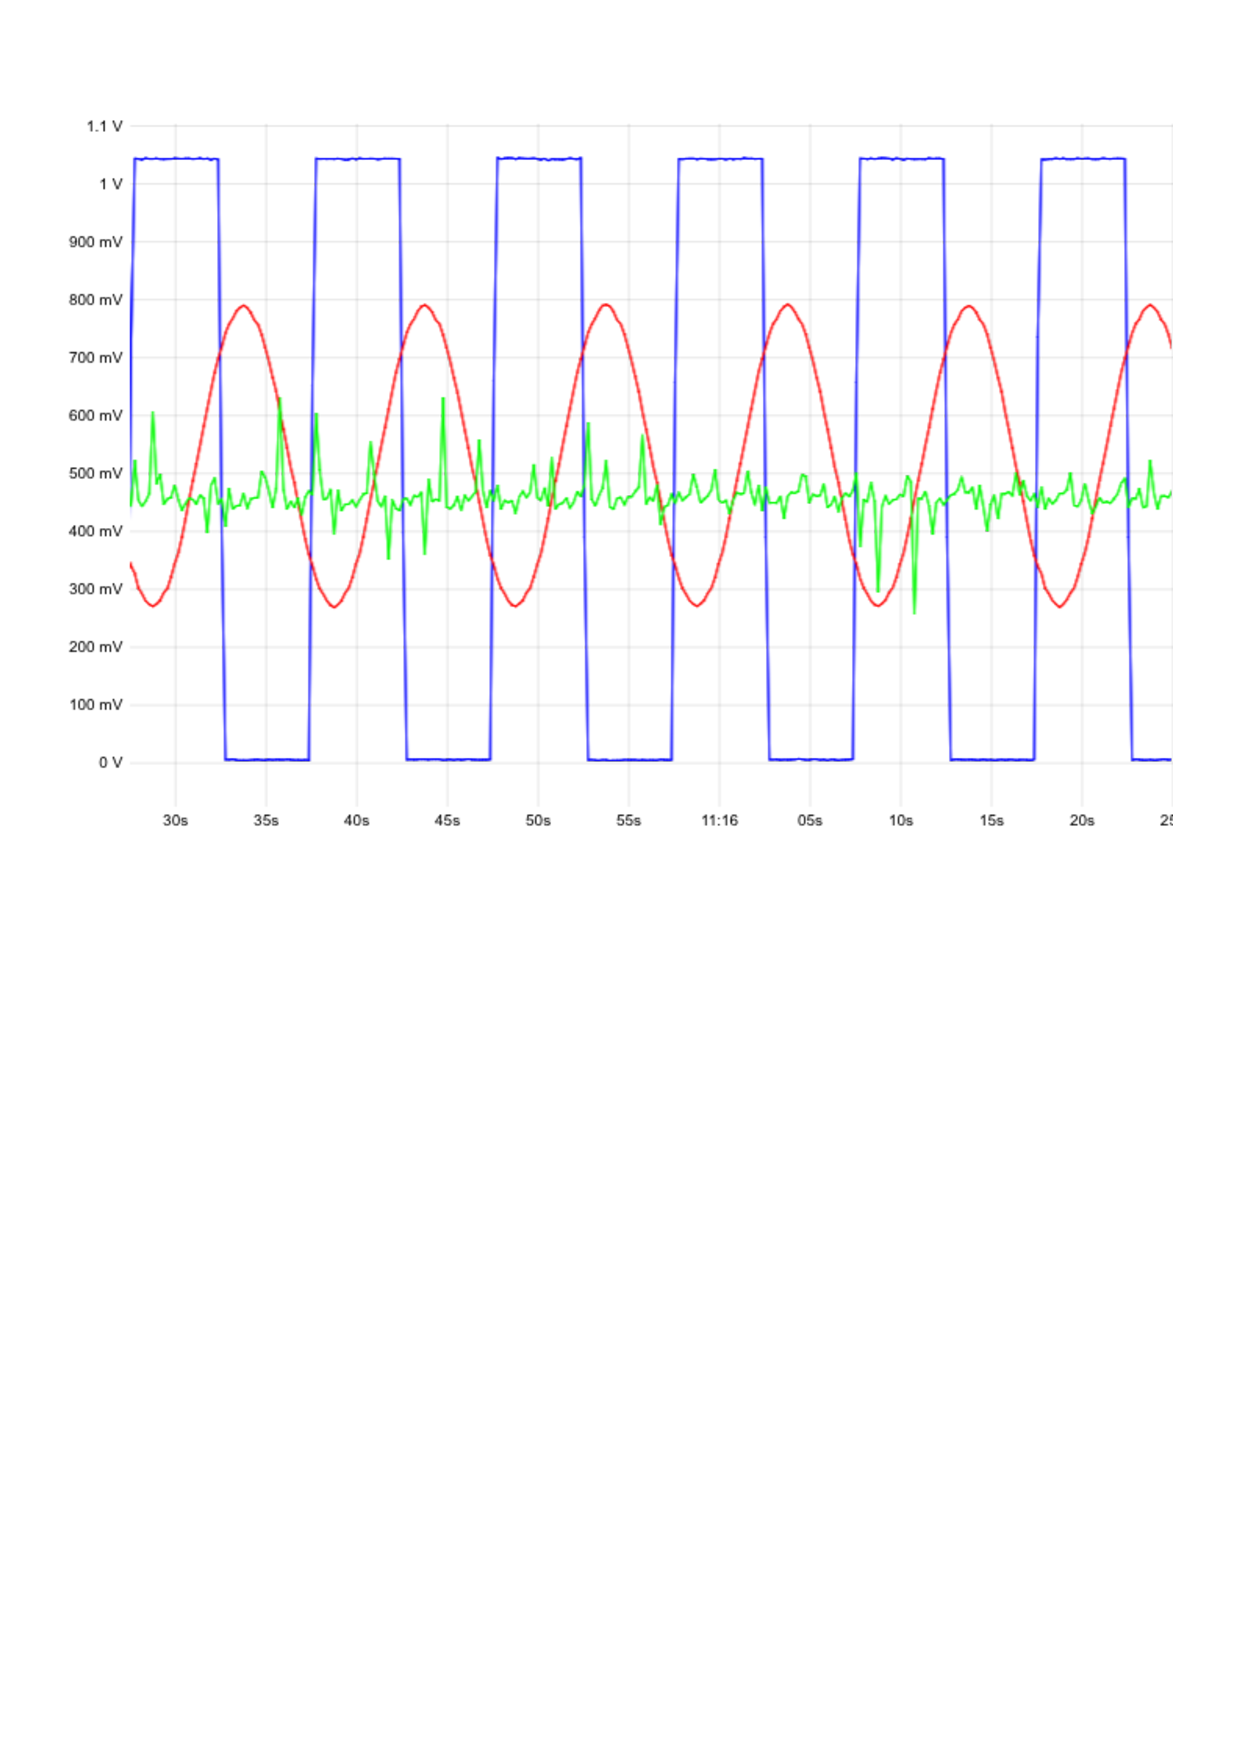
\includegraphics[trim={0cm 0cm 0cm  0cm}, clip, width=.9\textwidth]{./figures/standardsignals/picologChemComp.pdf}
\captionsetup{justification=centering}
\caption{Standard signals recorded using a PicoScope}
\label{fig: test1 picolog}
\end{figure}

\begin{figure}[h!]
\centering
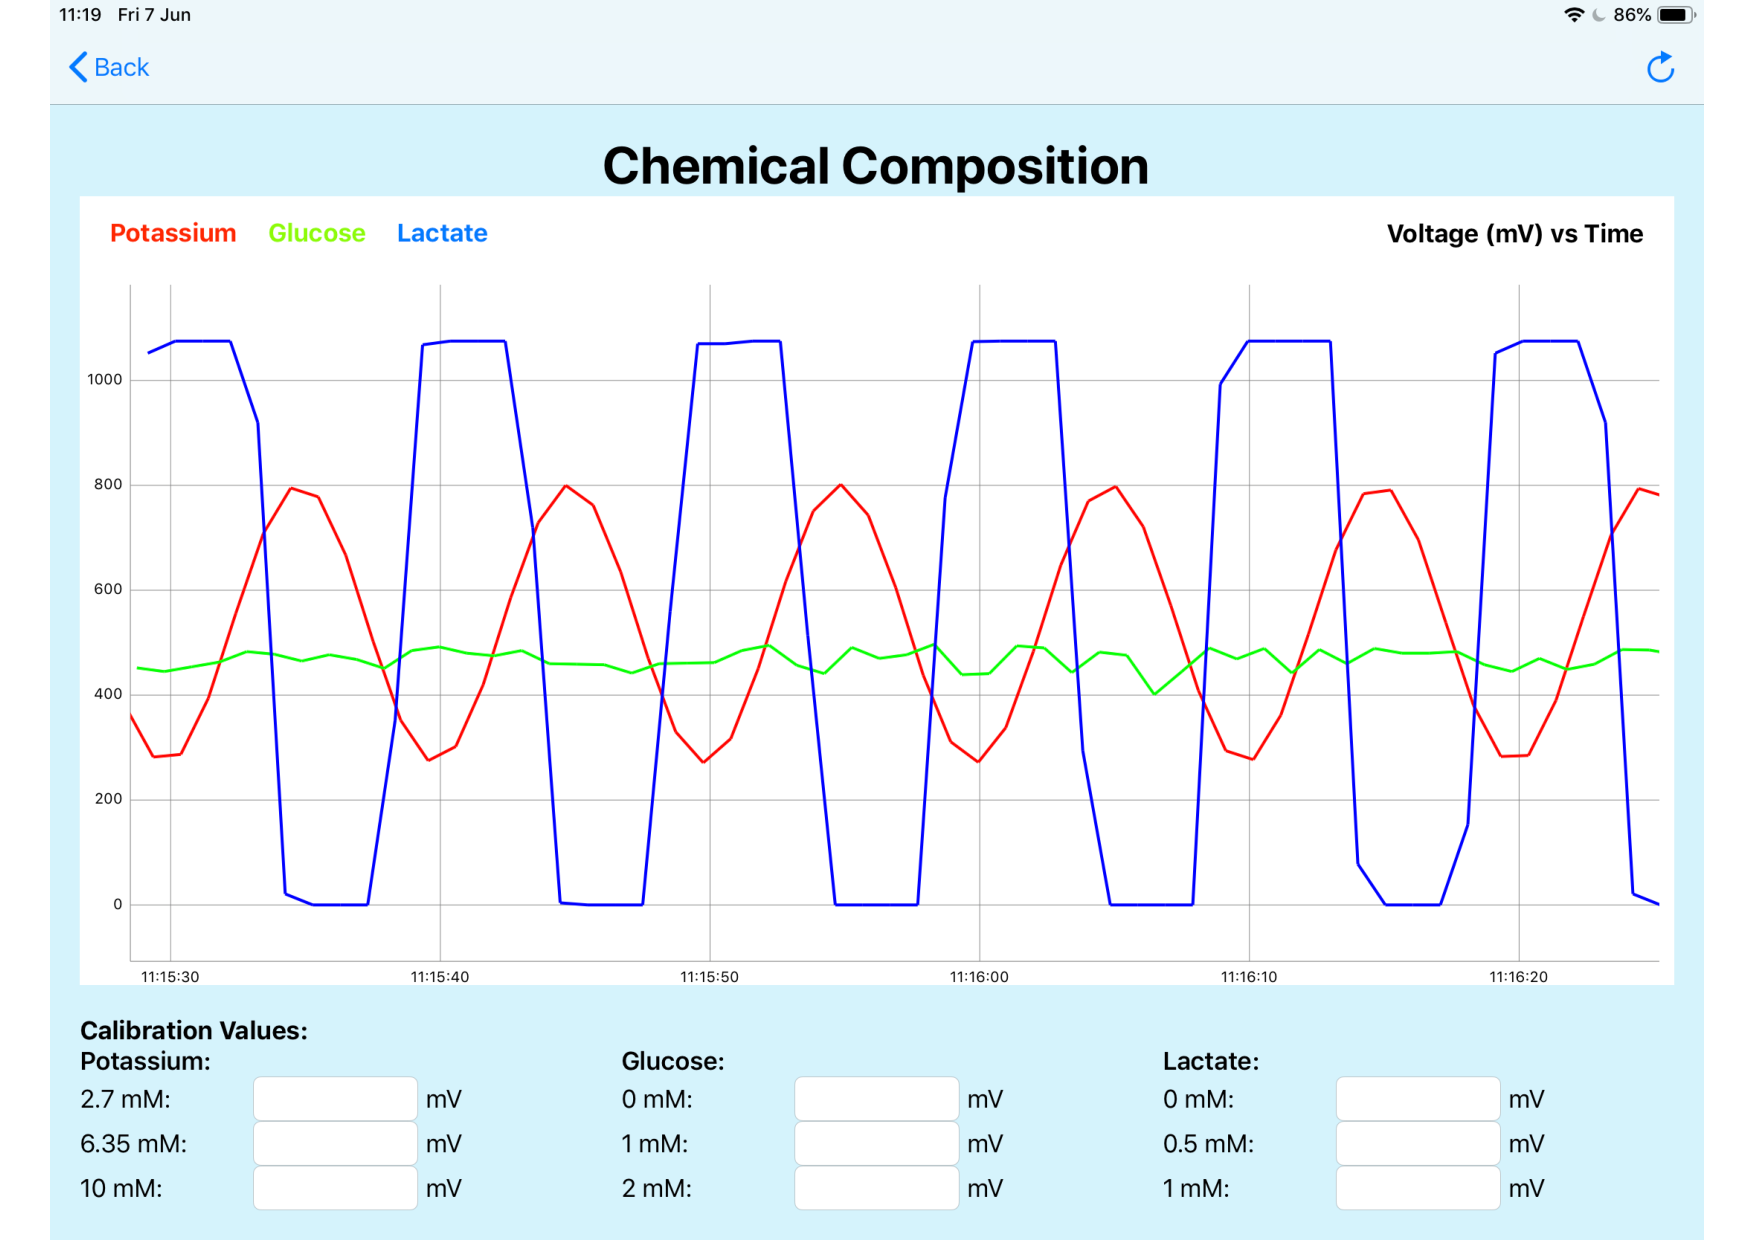
\includegraphics[trim={0cm 0cm 0cm  0cm}, clip, width=.9\textwidth]{./figures/standardsignals/appChemComp.pdf}
\captionsetup{justification=centering}
\caption{Standard signals recorded using the iPad app}
\label{fig: test1 app}
\end{figure}

Figure~\ref{fig: test1 picolog} shows the raw signals received on PicoLog, and Figure~\ref{fig: test1 app} shows the three signals received on the Chemical Composition page of the app after undergoing filtering and processing on the Arduino. 

Looking at the noise signal, shown in green on both plots, the raw signal in Figure~\ref{fig: test1 picolog} shows lots of sudden peaks. The app shows the noisy signal has been smoothed due to the filtering and averaging methods implemented. 

The raw square wave, shown in blue, has an instantaneous change between the two voltage levels. However, on the app, the change between the voltage levels is not sharp. The discontinuous nature of the square wave is not represented well on the app due to the block averaging method implemented. 

Comparing the sine waves, shown in red, the app shows a slightly more jagged signal. This is because the app has a lower sampling frequency of 1Hz, compared to the PicoScope's 5Hz sampling frequency. The higher frequency captures the signal better so results in a smoother wave. Regardless, the sine wave is  well represented on the app.

The peak amplitudes of the sine and square wave on the app match that recorded on PicoLog. However, it can be noted that between Figures~\ref{fig: test1 picolog} and \ref{fig: test1 app} there is a time lag of 1.25 seconds because of the delay incurred by wireless transmission.


\subsection{Spreading Depolarisation}